\chap{Zustand: Mach nicht immer dasselbe (fortgeschritten)}\label{ch.states}

Das Programm in VPL ist eine Liste von Ereignis-Aktions Paaren. Alle Ereignisse werde eins nach dem anderen überprüft, ob sie stattfinden und falls ja, wird die dazugehörige Aktion ausgelöst. Danach beginnt die Überprüfung von vorne. Wir möchten nun, dass einige Ereignis-Aktions Paare zu einer bestimmten Zeit aktiv sind und andere nicht. Zum Beispiel in Kapitel ~\ref{ch.line}, falls der Roboter vom Klebeband abkommt, möchten wir, dass er nach links oder nach rechts dreht, um das Klebeband zu suchen, je nach der Seite auf welcher er das Klebeband verloren hat.

Zustände werden im \emph{fortgeschrittenen} VPL Modus ausgeführt. Klick auf \blksm{advanced}, bevor du mit den folgenden Projekten arbeitest.

\sect{Klopf, klopf}

In vielen Programmen haben wir ein Schalter benutzt, um ein Verhalten des Roboters auszulösen und einen anderen, um dieses wieder zu stoppen. Stell Dir nun den Startschalter deines Computer vor. 
%\blksm{power-button}:
Hier wird derselbe Schalter benutzt, um diesen ein- oder auszuschalten. Der Schalter \emph{weiss} in welchem Zustand er sich gerade befindet: \bu{eingeschaltet} oder \bu{ausgeschaltet}. Der Schalter wird durch ein kleines grünes Licht beleuchtet, um anzuzeigen in welchem Zustand er sich gerade befindet.

Schreibe ein Programm, dass die Lichter des Roboters anstellt, falls er berührt wird und wieder abstellt, wenn er ein zweites Mal berührt wird.

{\raggedleft \hfill Program file \bu{tap-on-off.aesl}}

Das benötigte Verhalten wird in einem  \textit{Zustandsdiagramm} dargestellt:


\begin{center}
\begin{picture}(240,45)
%\put(0,0){\framebox(240,40){}}
\put(20,20){\circle{40}}
\put(0,0){\makebox(40,40){\textsf{aus}}}
\put(220,20){\circle{40}}
\put(200,0){\makebox(40,40){\textsf{ein}}}
\put(40,10){\vector(1,0){160}}
\put(0,10){\makebox(240,10){\textsf{klopfen $\rightarrow$ einschalten}}}
\put(200,30){\vector(-1,0){160}}
\put(0,30){\makebox(240,10){\textsf{klopfen $\rightarrow$ ausschalten}}}
\end{picture}
\end{center}

Im Diagramm sind zwei Zustände durch Kreise angezeigt, die mit den Namen des Zustandes \bu{eingeschaltet} und \bu{ausgeschaltet} angeschrieben sind. Der Roboter kann von dem Zustand  \bu{eingeschaltet} zum Zustand \bu{ausgeschaltet} und zurück wechseln, aber nur durch das Befolgen der Instruktionen die auf den Pfeilen angegeben sind. Diese Ereignis-Aktions Paare bedeuten:

\begin{itemize}

\item \emph{Falls} im Zustand \bu{ausgeschaltet} ein \emph{Klopfen}
sattfindet, $\rightarrow$ schalten die Lichter  \emph{ein} \textbf{\textit{und}} wechselt
der Zustand auf \bu{eingeschaltet}.

\item \emph{Falls} im Zustand \bu{eingeschaltet} ein \emph{Klopfen}
sattfindet, $\rightarrow$ schalten die Lichter  \emph{aus} \textbf{\textit{und}} wechselt
der Zustand auf \bu{ausgeschaltet}.

\end{itemize} 

Das fett hervorgehobene Wort ``\textbf{\textit{und}}'' vor dem Pfeil~$\rightarrow$ bedeutet, dass  es \emph{zwei Bedingungen} gibt, die wahr sein müssen, damit der Umschaltvorgang ausgeführt wird. (a) Der Roboter muss in einem bestimmten Zustand sein und (b) das Ereignis muss stattfinden. Wenn beide Bedingungen wahr sind, wird das Umschalten durchgeführt, dies führt dazu, dass der Status geändert und die Aktion ausgelöst wird, die nach dem Pfeil~$\rightarrow$ geschrieben steht.

Es ist wichtig zu verstehen, dass die zwei Teile der Bedingung unabhängig sind. In dem oben aufgeführten Diagramm (hier wiederholt):
\begin{center}
\begin{picture}(240,45)
\thicklines
%\put(0,0){\framebox(240,40){}}
\put(20,20){\circle{40}}
\put(0,0){\makebox(40,40){\textsf{aus}}}
\put(220,20){\circle{40}}
\put(200,0){\makebox(40,40){\textsf{ein}}}
\put(40,30){\vector(1,0){160}}
\put(0,30){\makebox(240,10){\textsf{klopfen $\rightarrow$ einschalten}}}
\put(200,10){\vector(-1,0){160}}
\put(0,10){\makebox(240,10){\textsf{klopfen $\rightarrow$ ausschalten}}}
\end{picture}
\end{center}

erscheint das Ereignis \emph{Klopfen} zweimal, aber die Aktion, ausgelöst durch das Stattfinden eines Ereignisses  \emph{hängt von} dem Zustand des Roboters ab, indem sich dieser gerade befindet.

Ähnlich, wie in einem Einzelzustand, können verschiedene Ereignisse verschiedene Aktionen auslösen und Umschaltungen in verschiedene neue Zustände bewirken, wie im folgenden Diagramm:

\begin{center}
\begin{picture}(240,80)
\thicklines
%\put(0,0){\framebox(240,80){}}
\put(30,42){\circle{30}}
\put(14,28){\makebox(30,30){\textsf{aus}}}
\put(220,22){\circle{30}}
\put(205,8){\makebox(30,30){\textsf{ein2}}}
\put(40,57){\vector(1,0){160}}
\put(220,60){\circle{30}}
\put(205,45){\makebox(30,30){\textsf{ein1}}}
\put(40,27){\vector(1,0){160}}
\put(0,60){\makebox(240,10){\textsf{linker Knopf $\rightarrow$ leuchte grün}}}
\put(0,30){\makebox(240,10){\textsf{rechter Knopf$\rightarrow$ leuchte rot}}}
\end{picture}
\end{center}

Das Drücken des linken Knopfs während dem Zusand \textbf{aus} führt dazu, dass ein grünes Licht eingeschaltet wird und der Zustand wechselt zu Zustand \textbf{ein1}, während das Drücken des rechten Knopfes  \emph{im selben Zustand} dazu führt, dass eine andere Aktion ausgelöst wird, nähmlich dass ein rotes Licht eingeschaltet wird und der Zustand in einen anderen Zustand, nähmlich Zustand \textbf{ein2} wechselt.

\sect{Die Umsetzung Zustandsdiagramme mit Ereignis-Aktions-Paare}

\Cref{fig.turn-on-off} zeigt die Durchführung des beschriebenen Verhaltens in der Zustandsmaschine als Ereignis-Aktions-Paaren.

\begin{figure}
	\subfigure[Klopfe, um ein - und auszuschalten]{
		\label{fig.turn-on-off1}
		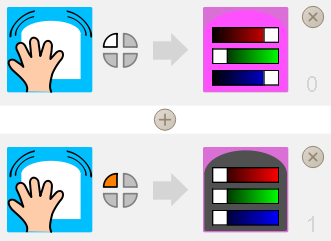
\includegraphics[width=.4\textwidth]{tap-on-off1}
	}
	\hfill
	\subfigure[Klopfe, um den Zustand zu wechseln]{
		\label{fig.turn-on-off2}
		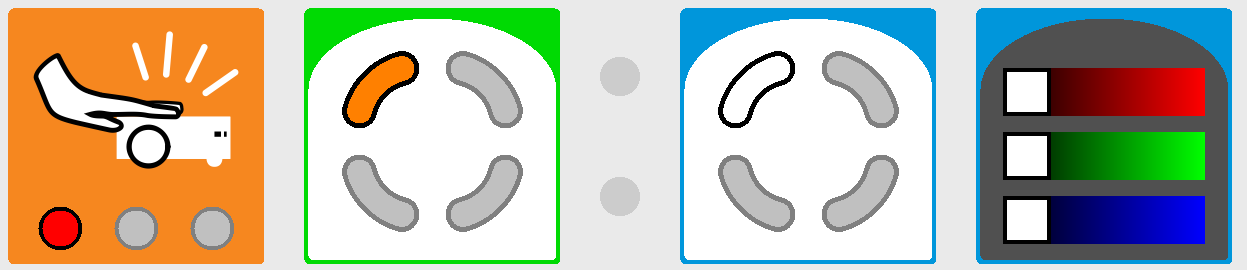
\includegraphics[width=.4\textwidth]{tap-on-off2}
	}
	\caption{Klopfen führt zu verschieden Resultaten abhängig vom Zustand}
	\label{fig.turn-on-off}
\end{figure}


Im ersten Ereignis-Aktions Paar, ist das Ereignis zusammengesetzt aus dem Berührungsblock und der Anzeige des Zustandes \blksm{tap-turn-on-state-only}: 
\blkc{tap-turn-on}

Die Zustände werden durch die Viertel eines Kreises angezeigt. Jedes Viertel kann entweder eingeschaltet (orange) oder ausgeschaltet (weiss) sein. Wir benützen das linke obere Viertel, um anzuzeigen, ob die Lichter eingeschaltet oder ausgeschaltet sind. Bei diesem Paar ist das linke obere Viertel weiss. Das bedeutet, dass der Zustand auf ausgeschaltet steht. Die Bedeutung von dieser Paar ist, dass falls der Roboter berührt wird und die Lichter ausgeschaltet sind, diese eingeschaltet werden.

Ähnlich bedeutet das zweite Ereignis-Aktions Paar, dass falls der Roboter berührt wird und die Lichter an sind, diese abgeschaltet werden:
\blkc{tap-turn-off} 
%Das Viertel ist dabei orange, was bedeutet, dass der Zustand auf eingeschaltet steht.

Wenn du das Zusstandsdiagramm des Roboters betrachtest, wirst du bemerken, dass erst die Hälfte der Arbeit erledigt ist. Beim Ein- und Ausschalten der Lichter müssen ebenfalls die Zustände des Roboters geändert werden von \bu{eingeschaltet} auf  \bu{ausgeschaltet}. Dazu schreiben wir zwei zusätzliche Ereignis-Aktions Paare und benutzen dazu den Aktionsblock Zustand \blksm{action-states} (\cref{fig.turn-on-off2}).

Die Bedeutung von der folgende Paar ist: \emph{Falls} der Roboter berührt wird
im Zustand \bu{ausgeschaltet}, ändere den Zustand auf \bu{eingeschaltet}:
\blkc{tap-state-on}
Die Bedeutung von der folgende Paar ist: \emph{Falls} der Roboter berührt wird im Zustand \bu{eingeschaltet}, ändere den Zustand auf \bu{ausgeschaltet}: \blkc{tap-state-off}

Bezogen auf das ganze Programm, welches aus den vier Paaren aus der \cref{fig.turn-on-off}  zusammengesetzt ist, sehen wir, dass jedes Ereignis zwei Aktionen auslöst: Einschalten des Lichts und Änderung des Zustands des Roboters. Beides, die Aktion und die Änderung des Zustandes hängt vom Zustand des Roboters ab, in welchem er sich gerade befindet. Dieser Zustand wird \emph{IST-Zustand} genannt.

\sect{In wie vielen verschiedenen Zuständen kann sich der  Roboter befinden?}

Die Zustände werden durch die Viertel eines Kreises angezeigt. Sowohl als Ereignis, als auch im Zustands Aktionsblock kann jedes Viertel folgende Bedeutung haben. 
\begin{itemize}

\item Weiss: Das Viertel befindet sich im Zustand \emph{ausgeschaltet};
\item Orange: Das Viertel befindet sich im Zustand \emph{eingeschaltet};
\item Grau: das Viertel wird nicht berücksichtigt;

\end{itemize}

Bei \blksm{states} sind das linke obere und das rechte untere Viertel im Zustand eingeschaltet. Das Viertel rechts oben ist auf dem Zustand ausgeschaltet und das Viertel links unten wird nicht berücksichtigt. Das bedeutet, dass falls \blksmpure{states} mit dem Ereignisblock verbunden ist, ein Ereignis stattfindet, falls die Zustände auch wie folgt gesetzt sind:

\begin{center}
\centering \makebox{\raisebox{-1.7em}{
\includegraphics[height=4em]{states1}}}\quad or \quad \makebox{\raisebox{-1.7em}{
\includegraphics[height=4em]{states2}}}
\end{center}

Da jedes der vier Viertel entweder ein- oder ausgeschaltet sein kann, sind 2 $\times$ 2 $\times$ 2 $\times$ 2 = 16 verschiedene Zustände möglich.

\begin{quote}
\bu{(aus, aus, aus, aus)\\(aus, aus, aus, ein)\\(aus, aus, ein, aus)\\
\mbox{}\hspace{3em}\ldots\\
(ein, ein, ein, aus)\\
(ein, ein, ein, ein)}.
\end{quote}
\Cref{fig.all-states} zählt all die Zustände graphisch auf. 

\importantbox{Der Ist-Zustand des Roboters wird im Kreis der LED Lampen auf der Oberseite des Computers angezeit. \cref{fig.state-leds} zeigt den Roboter mit den Zuständen \bu{(ein, ein,
ein, ein)}}

\trickbox[Information]{Wird ein Programm gestartet, sind die ursprünglichen Zustände
\bu{(aus, aus, aus, aus)}: \blk{state-all-off}.}

\trickbox{Falls du nicht alle 16 verschiedene Zustände benötigst, sondern z.B. nur 2 oder 4, bist du frei zu entscheiden, welche Viertel du benütztst, um deine Zustände wiederzugeben. Zusätzlich, wenn du zwei verschiedene Dinge programmierts und jeder hat davon zwei mögliche Werte, kannst du zwei Viertel unabhänig voneinander benutzen. Deshalb ist die Wahlmöglichkeit \emph{nicht berücksichtigen} so nützlich!
}

\begin{figure}
	\subfigure[Alle möglichen Züstande von Tyhmio]{
		\label{fig.all-states}
		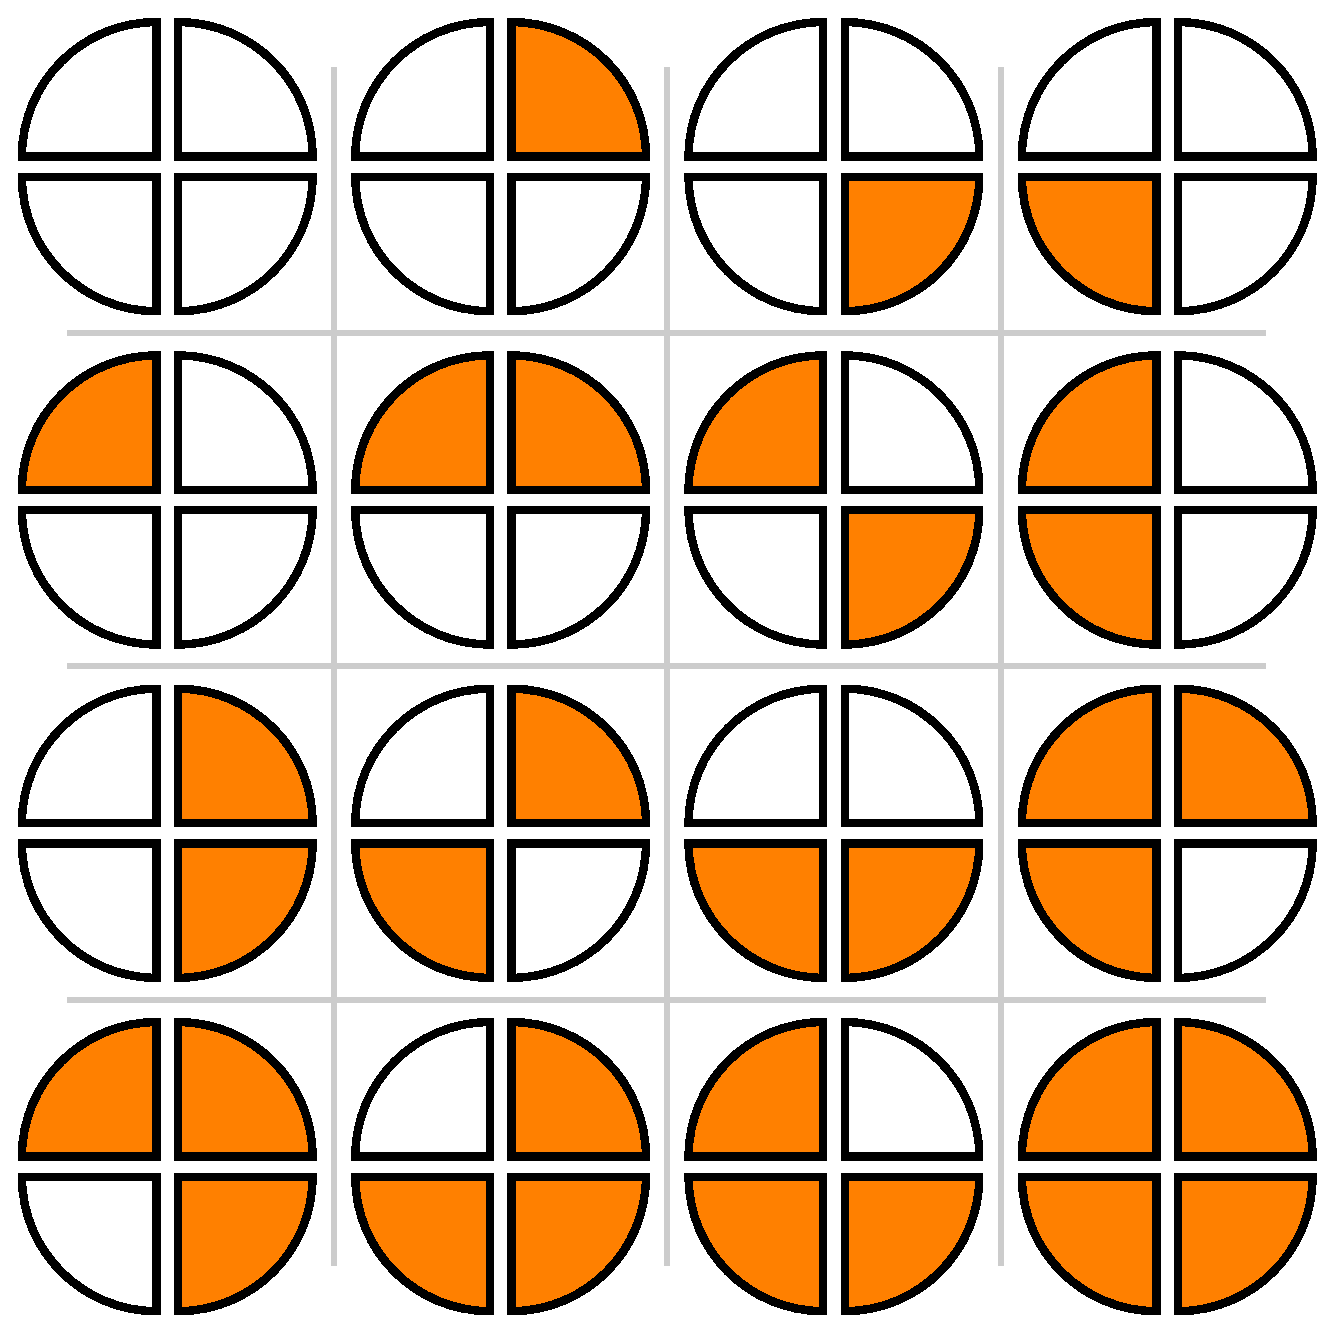
\includegraphics[width=.4\textwidth]{all-states}
	}
	\hfill
	\subfigure[Der LED Kreis zeigt, die unterschiedlichen Zustände auf]{
		\label{fig.state-leds}
		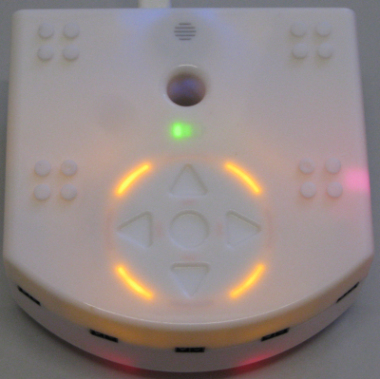
\includegraphics[width=.4\textwidth]{state-leds}
	}
	\caption{Die Zustände von Tymio und deren Repräsentation}
\end{figure}


\sect{Erwische die Maus}

Schreibe ein Programm, dass den Roboter nach links und rechts drehen lässt, um eine Maus zu suchen. Wird eine Maus mit dem äussersten linken Sensor entdeckt, wird die Suche fortgesetzt, bis die Maus von dem äussersten rechten Sensor entdeckt wird. Nun ist die Position des Roboters genau gegenüber der Maus (\cref{fig.cat-mouse}).

{\raggedleft \hfill Program file \bu{mouse.aesl}}

\begin{figure}
	\subfigure[Die Katze hat die Maus gefunden]{\label{fig.cat-mouse}
	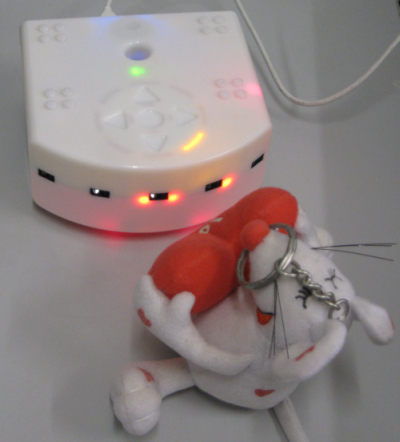
\includegraphics[width=0.4\textwidth]{cat-mouse}}
	\hfill
	\subfigure[Suchen mit dem äußersten rechten Sensor]{\label{fig.mouse2}
	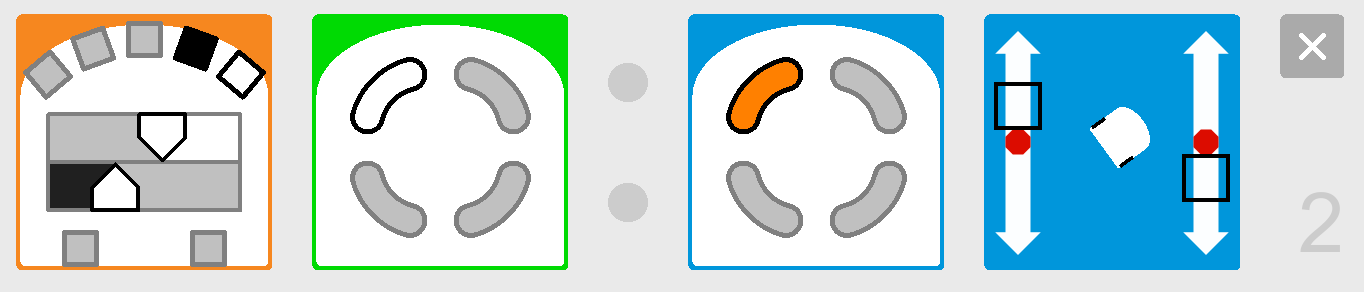
\includegraphics[width=0.4\textwidth]{mouse2}}
	\caption{Der Roboter Katze ist für die Maus suchen}
\end{figure}

Das Ereignis-Aktions Paar
\blkc{mouse1}
führt dazu, dass der Roboter nach links abdreht. Dies findet nur statt, falls das linke obere Viertel im Zustand ausgeschaltet ist. Am Anfang sind alle Zustände auf ausgeschaltet.


Das erste Ereignis-Aktions Paar in \cref{fig.mouse2} wartet bis die Maus mit dem äussersten linken Sensor entdeckt wird. Beachte, dass das schmale Quadrat daneben weiss ist, sodass das Ereignis nur stattfindet, falls nur der äusserste rechte Sensor eine Maus erkennt. Das Zweite Ereignis-Aktions Paar in der Abbildung ändert den Zustand \cref{fig.mouse2}.

Das letzte Ereignis-Aktions Paar im Programm ist
\blkc{mouse3}
Dieses bewirkt, dass der Roboter stoppt, falls die Maus direkt vor dem mittleren Sensor zu liegen kommt.

Warum muss das Ereignis dieses Paares von einem Zustand abhängig sein? Der Grund ist, dass der mittlere Sensor die Maus auch beim Scan von links nach rechts erkennen wird. Wir wollen, dass der Roboter jedoch einen vollen Scan vollbringt, bevor er zur Position der Maus zurückkehrt. Deshalb ist es notwendig, dass diese erste Entdeckung der Maus ignoriert wird. Dies wird erreicht, indem der Scan erst gestoppt wird, falls der Zustand auf \bu{eingeschaltet} und dieser erst beim Abschluss des vollständigen Scans auf eingeschaltet geändert wird.

\trickbox{Experimentiere mit der Position der Maus. Ist diese zu nahe am Roboter, werden die Sensoren zu beiden Seiten die Maus ebenfalls erkennen. Das Ereignis findet jedoch nur statt, wenn die äusseren Sensoren die Maus  \emph{nicht} erkennen}

\vfill
\vfill

\exercisebox{\thechapter.1}{
Schreibe ein Programm, das den Roboter tanzen lässt: Der Roboter soll für zwei Sekunden nach links und dann für drei Sekunden nach rechts drehen. Diese Bewegung soll unendlich oft wiederholt werden.}

\vfill

\exercisebox{\thechapter.2 (schwierig)}{
Verändere das Folge der Linie Program aus dem \cref{ch.line} so, dass der Roboter nach links dreht, falls dieser die Linie auf die rechte Seite verlässt und nach rechts dreht, falls dieser die Linie auf die linke Seite verlässt.
}